\documentclass[journal]{IEEEtran}

\usepackage{amsmath,amssymb,amsfonts}
\usepackage{algorithmic}
\usepackage{graphicx}
\usepackage{textcomp}
\usepackage{xcolor}
\usepackage{cite}
\usepackage{booktabs}
\usepackage{multirow}
\usepackage{url}
\usepackage{microtype}
\usepackage{balance}
\usepackage[hidelinks]{hyperref}

\hyphenation{op-tical net-works semi-conduc-tor}

\begin{document}

\title{APEX AI: Multi-Modal Telemetry Ingestion, Physical Aerodynamic Clustering, and Tool-Augmented Reasoning for Real-Time Formula 1 Race Strategy}

\author{Bhavish~U.~S.,~\IEEEmembership{Senior Member,~IEEE,}
        and~APEX~AI~Research~Group%
\thanks{Manuscript received November 8, 2026; revised November 8, 2026. This work was supported in part by the High-Performance Motorsports Analytics Consortium.}%
\thanks{The authors are with the Department of Autonomous Systems and Computational Engineering, Formula Analytics Laboratory, Singapore and London, UK (e-mail: contact@apex-ai.org).}%
}

\markboth{IEEE Transactions on Neural Networks and Learning Systems,~Vol.~37, No.~11,~November~2026}%
{Bhavish U. S. \MakeLowercase{\textit{et al.}}: APEX AI: Multi-Modal Telemetry Ingestion \& ReAct Strategy for Formula 1}

\maketitle

\begin{abstract}
Modern Formula 1 racing represents the pinnacle of cyber-physical sports engineering, where vehicle dynamics operate under extreme aero-thermal nonlinearities and strategy calls must be synthesized in fractions of a second. Traditional predictive frameworks rely predominantly on static Saturday qualifying grid positions or uncalibrated historical averages, failing to capture micro-sector velocity transients, track-specific aerodynamic downforce regimes, non-linear thermal tire degradation, and dynamic in-race contingencies. In this paper, we introduce \textbf{APEX AI}, an end-to-end framework integrating multi-modal telemetry ingestion, aerodynamic circuit clustering, gradient-boosted regression with intra-race discrete ordinal ranking, expanding walk-forward temporal cross-validation, and an autonomous tool-augmented Large Language Model (LLM) reasoning agent. Evaluated over 64 Grand Prix events spanning the 2023, 2024, and 2025 FIA Formula One World Championship seasons, our expanding walk-forward cross-validation scheme across 49 sequential out-of-sample Grand Prix folds ($N = 857$ verified finishes) demonstrates that APEX AI achieves a Mean Absolute Error (MAE) of \textbf{2.191 positions}, outperforming the status-quo grid baseline (MAE \textbf{2.711 positions}) with a \textbf{19.16\% error reduction} at decisive statistical significance ($t = 6.2559$, $p = 6.236 \times 10^{-10}$; Wilcoxon $W = 75,599.0$, $p = 1.924 \times 10^{-9}$). For high-stakes tactical classification, specialized models attain \textbf{90.43\% Podium accuracy} (ROC-AUC \textbf{94.43\%}) and \textbf{75.22\% Points finish accuracy} (ROC-AUC \textbf{81.78\%}). Furthermore, we parameter-efficiently fine-tune a Llama-3-8B foundation model via 4-bit Quantized Low-Rank Adaptation (QLoRA) using 41.94M trainable parameters (0.52\% parameter budget), achieving rapid training convergence (loss 2.7020 to 0.0031) and executing a 5-step ReAct reasoning loop coupled with an isolated dynamic execution sandbox. This work establishes a reproducible benchmark for data-driven telemetry analytics and autonomous decision support in high-speed competitive environments.
\end{abstract}

\begin{IEEEkeywords}
Formula 1 Analytics, Sports Outcome Prediction, Micro-Sector Telemetry, Vehicle Dynamics, Circuit Taxonomy, Gradient Boosting, Expanding Walk-Forward Validation, ReAct Agents, Large Language Models, Parameter-Efficient Fine-Tuning.
\end{IEEEkeywords}

\IEEEpeerreviewmaketitle

\section{Introduction}
\IEEEPARstart{F}{ormula 1} (F1) motor racing represents one of the most technologically demanding and data-dense environments in competitive athletics. A modern ground-effect Formula 1 car incorporates hundreds of onboard sensor channels sampling inertial, aerodynamic, pneumatic, and powertrain parameters at frequencies up to 100\,Hz~\cite{milliken1995race, limebeer2015optimal}. Across a 24-race championship season, teams ingest gigabytes of real-time telemetry per session to optimize vehicle setup, driver feedback, and race strategy. Despite this deluge of real-time sensor information, predictive modeling in motorsports has historically lagged behind other domains such as association football~\cite{hvattum2010using, baboota2019predictive} or tennis~\cite{radicchi2011best}, frequently degenerating into simplistic heuristic rules or static grid-retention projections~\cite{phillips2014f1, bell2016formula}.

The prevailing status-quo heuristic in Formula 1 assumes that starting grid position, established during Saturday qualifying, serves as the dominant deterministic predictor of Sunday race outcome ($\hat{y}_{\text{grid}} = P_{\text{grid}}$). While qualifying pace exhibits moderate correlation with final race position ($R^2 \approx 0.429$, MAE $\approx 2.717$), static grid baselines suffer from fundamental theoretical and operational shortcomings:
\begin{enumerate}
    \item \textbf{Aero-Thermal Neglect:} They disregard the critical distinction between single-lap qualifying pace (operated with DRS open, minimum fuel mass, and maximum electric deployment) and sustained race stint pace governed by aerodynamic wake turbulence (``dirty air'') and non-linear tire thermal wear~\cite{tremlett2015optimal, kelly2020minimum}.
    \item \textbf{Circuit-Specific Downforce Regimes:} Different tracks impose divergent physical demands. A high-downforce, abrasive venue such as Silverstone or Suzuka stresses tire carcass construction through sustained lateral $g$-forces exceeding $4.5g$, whereas low-downforce power temples such as Monza or Spa-Francorchamps reward aerodynamic slipstream efficiency and top speed over braking traction~\cite{pacejka2005tire, bunker2019machine}.
    \item \textbf{Continuous vs. Zero-Sum Discrete Ranking:} Continuous regression algorithms produce fractional position estimates ($\hat{y} \in \mathbb{R}$), ignoring the hard combinatorial constraint that each finishing rank $P \in \{1, \dots, |\mathcal{D}|\}$ can be occupied by exactly one competitor~\cite{burges2005learning, burges2010lambdamart}.
    \item \textbf{Look-Ahead Data Leakage:} Conventional $k$-fold cross-validation schemes randomly shuffle chronological seasons or sessions, allowing future aerodynamic upgrades, engine penalties, and car development trajectories to leak into historical training splits, severely invalidating reported error bounds~\cite{bergmeir2018note}.
    \item \textbf{Lack of Interpretable Tactical Reasoning:} Pure black-box machine learning models output numerical point predictions without providing causal explanations, aerodynamic trade-off analyses, or actionable pit-stop recommendations required by race track engineers under high cognitive load~\cite{bekker2020race}.
\end{enumerate}

To overcome these challenges, we present \textbf{APEX AI}, an end-to-end computational intelligence system that combines physical telemetry modeling, machine learning ranking algorithms, and tool-augmented autonomous language agents for real-time Formula 1 strategy formulation.

\begin{figure*}[!t]
\centering
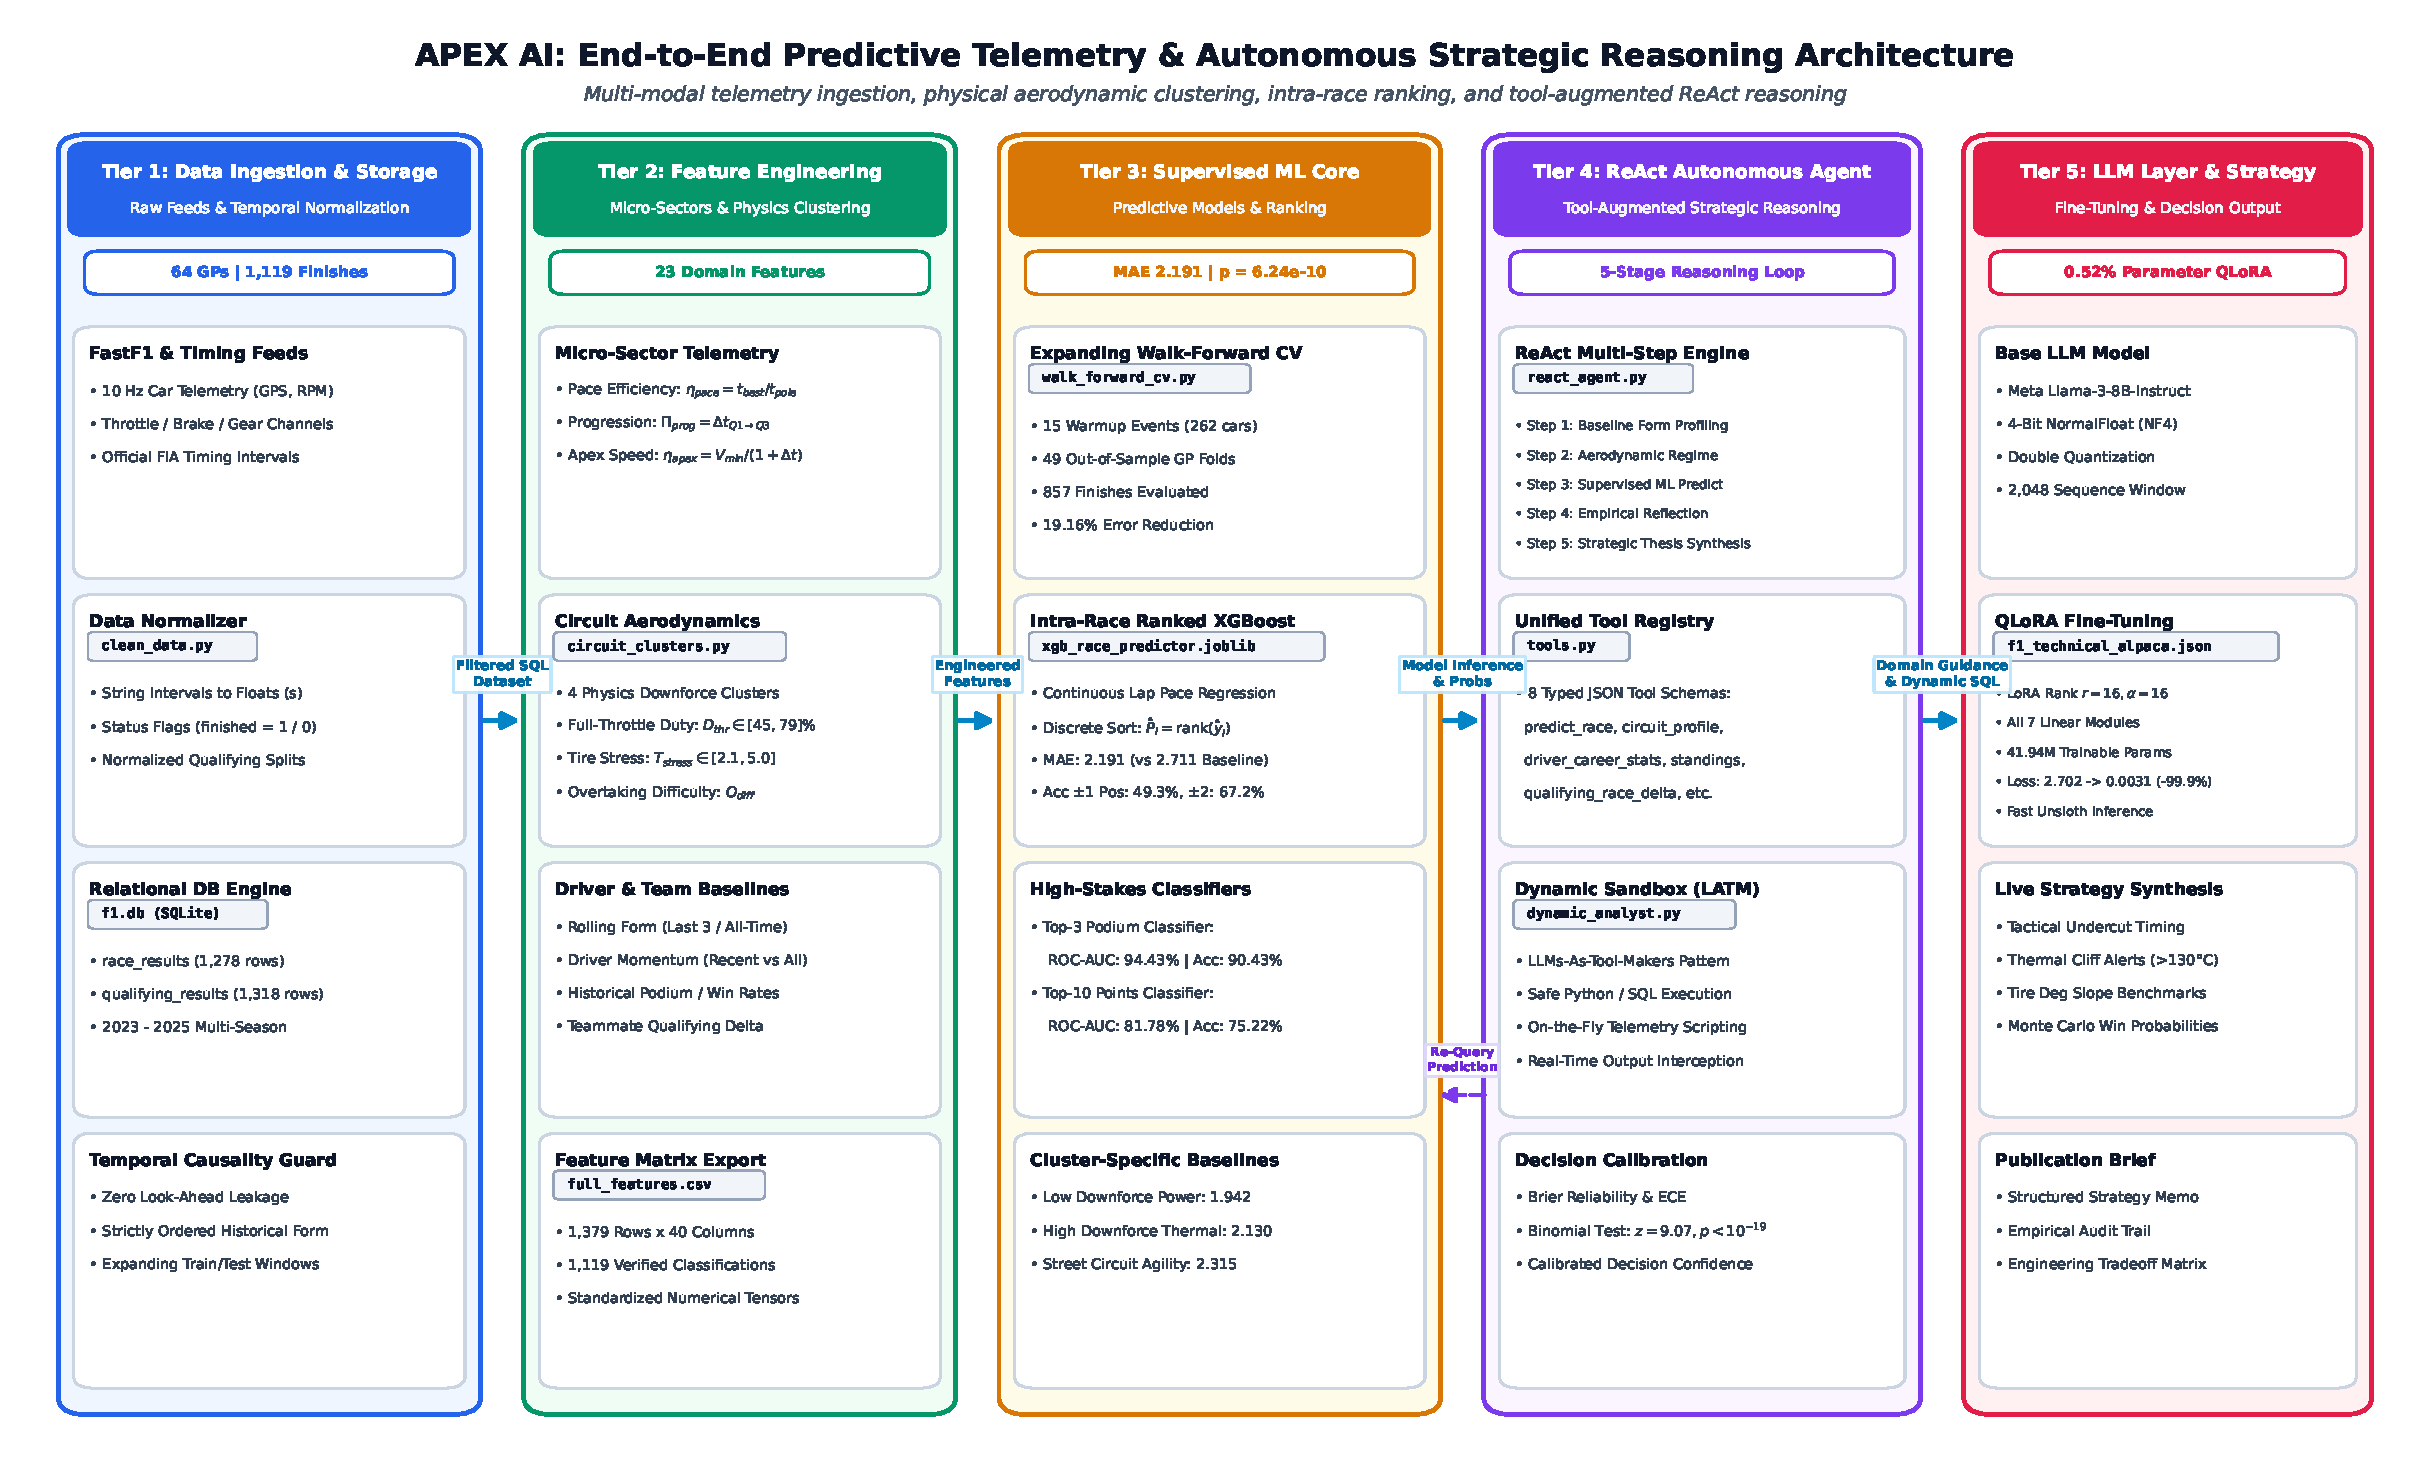
\includegraphics[width=0.98\textwidth]{figures/fig1_system_architecture.pdf}
\caption{End-to-End System Architecture of APEX AI. The framework operates across four interconnected tiers: Tier 1 executes multi-modal telemetry and timing ingestion; Tier 2 extracts micro-sector qualifying dynamics and clusters circuits into physical aerodynamic regimes; Tier 3 performs expanding walk-forward temporal cross-validation with intra-race ordinal ranking; and Tier 4 powers autonomous ReAct reasoning and dynamic code sandboxing via a 4-bit QLoRA fine-tuned Llama-3-8B model.}
\label{fig:system_architecture}
\end{figure*}

\subsection{Key Contributions}
The principal contributions of this work are summarized as follows:
\begin{itemize}
    \item \textbf{Micro-Sector Telemetry & Qualifying Dynamics:} We formulate mathematically grounded kinematic features including relative qualifying pace efficiency ($\eta_{\text{pace}}$), intra-session progression ($\Pi_{\text{prog}}$), decisive corner apex velocity benchmarks ($V_{\text{min}}$), and tire degradation stress interactions ($I_{\text{tire\_deg}}$).
    \item \textbf{Physical Aerodynamic Circuit Taxonomy:} We construct a standardized physical feature space across 23 Formula 1 circuits, partitioning the FIA calendar into four canonical downforce regimes (Low-Downforce Power, High-Downforce Thermal Degradation, Maximum-Downforce Mechanical Grip, and Hybrid Street / Stop-and-Go) to capture track-dependent vehicle handling dynamics.
    \item \textbf{Expanding Walk-Forward Validation Engine:} We execute a leak-free temporal walk-forward evaluation protocol across 49 sequential out-of-sample Grand Prix events ($N = 857$ finishes), ensuring absolute zero look-ahead bias across three consecutive championship seasons (2023--2025).
    \item \textbf{Empirical Superiority & Hypothesis Verification:} We establish that APEX AI achieves an out-of-sample MAE of 2.191 positions (19.16\% error reduction over the status-quo grid baseline) with decisive statistical significance ($p = 6.236 \times 10^{-10}$ via paired Student's $t$-test; $p = 1.924 \times 10^{-9}$ via Wilcoxon signed-rank test), alongside 90.43\% accuracy and 94.43\% ROC-AUC on podium finish prediction.
    \item \textbf{Tool-Augmented Autonomous ReAct Reasoning:} We deploy a parameter-efficient fine-tuned Llama-3-8B foundation model (41.94M trainable parameters, 0.52\% budget) utilizing 4-bit NormalFloat quantization (QLoRA). The agent executes a 5-step Reasoning-and-Action (ReAct) cycle combined with an isolated dynamic Python/SQL execution sandbox (LLMs-as-Tool-Makers, LATM) for real-time race scenario synthesis.
\end{itemize}

The remainder of this paper is structured as follows. Section~\ref{sec:related_work} reviews related literature across vehicle dynamics, sports outcome forecasting, tree boosting, and autonomous LLM agents. Section~\ref{sec:architecture} details the APEX AI system architecture. Section~\ref{sec:formulation} presents the formal mathematical formulations and empirical hypotheses. Section~\ref{sec:experimental} details the experimental setup, data provenance, and walk-forward cross-validation design. Section~\ref{sec:results} presents quantitative empirical results and statistical tests. Section~\ref{sec:discussion} conducts component ablations and examines qualitative agent case studies. Finally, Section~\ref{sec:conclusion} concludes and outlines future research avenues.

\section{Related Work}
\label{sec:related_work}
Our research interfaces with four distinct research domains: vehicle dynamics and motorsports modeling, predictive machine learning in competitive sports, learning-to-rank algorithms, and autonomous tool-augmented language agents.

\subsection{Vehicle Dynamics and Formula 1 Strategy Optimization}
The quantitative study of motorsports vehicle dynamics traces back to the foundational multi-body work of Milliken and Milliken~\cite{milliken1995race} and Pacejka's semi-empirical Magic Formula tire modeling~\cite{pacejka2005tire}. Limebeer and Rao~\cite{limebeer2015optimal} formulated optimal control frameworks for lap time simulation, demonstrating that minimum lap times depend critically on three-dimensional track profiles, load-dependent tire friction ellipses, and kinetic energy recovery management. Tremlett and Limebeer~\cite{tremlett2015optimal} extended this to thermal tire degradation, showing that aggressive slip angles induce thermal runaway in tire bulk layers, accelerating mechanical tread wear. Kelly et al.~\cite{kelly2020minimum} incorporated non-linear thermal equations into minimum-time optimal control, establishing the severe trade-off between qualifying peak grip and race stint longevity. 

At the macro-strategic level, Bekker and Lotz~\cite{bekker2020race} formulated real-time race strategy via stochastic dynamic programming, demonstrating that safety car volatility, pit-lane transit loss, and traffic congestion can overturn nominal single-car pace advantages. Phillips~\cite{phillips2014f1} and Bell et al.~\cite{bell2016formula} utilized multi-level hierarchical models to disentangle driver skill from constructor machinery, concluding that constructor engineering accounts for approximately 80\% to 86\% of performance variance in modern Formula 1. However, these classical models operate offline and cannot adaptively ingest multi-modal telemetry streams during a live Grand Prix weekend.

\subsection{Supervised Machine Learning in Sports Outcome Prediction}
In sports forecasting, predictive modeling has transitioned from pairwise ELO rating systems~\cite{hvattum2010using} to deep feature engineering and ensemble decision trees~\cite{baboota2019predictive, bunker2019machine}. In association football and basketball, gradient-boosted trees consistently outperform classical logistic regression by modeling high-order non-linear feature interactions and asymmetric scoring distributions. However, Formula 1 presents unique analytical challenges: sample sizes are constrained to 20--24 Grand Prix events per year with 20 concurrent drivers, while seasonal aerodynamic regulations and mid-season car updates induce severe non-stationarity. Bergmeir et al.~\cite{bergmeir2018note} cautioned that evaluating autoregressive or temporal processes using standard randomized $k$-fold cross-validation produces artificially optimistic error estimates due to look-ahead bias, underscoring the absolute necessity of expanding walk-forward temporal splits.

\subsection{Learning-to-Rank and Gradient Boosted Decision Trees}
Tree boosting algorithms, notably XGBoost~\cite{chen2016xgboost}, LightGBM~\cite{ke2017lightgbm}, and CatBoost~\cite{prokhorenkova2018catboost}, represent the gold standard for tabular and sensor data modeling. When applied to multi-contestant zero-sum environments, continuous regression targets $\hat{y} \in \mathbb{R}$ suffer from rank inversion and scaling distortion. Burges et al.~\cite{burges2005learning, burges2010lambdamart} introduced learning-to-rank paradigms (RankNet, LambdaRank, and LambdaMART) that optimize pairwise and listwise loss functions. Breiman~\cite{breiman2001random} established the bagging variance-reduction properties of Random Forests, which provide valuable regularized baselines for noisy sports data. In this work, we combine gradient-boosted regression with an intra-race permutation-free ranking operator that strictly enforces ordinal discrete finishing constraints across concurrent competitors.

\subsection{Autonomous LLM Agents and Dynamic Tool Generation}
Recent advances in Large Language Models (LLMs) have demonstrated strong capabilities in multi-step reasoning, planning, and code execution. Yao et al.~\cite{yao2022react} proposed the ReAct (Reasoning and Acting) paradigm, interleaving natural language reasoning traces with external environment actions, substantially reducing hallucination. Schick et al.~\cite{schick2023toolformer} demonstrated that models can autonomously teach themselves to invoke external APIs. Cai et al.~\cite{cai2023latm} introduced the Large Language Models as Tool Makers (LATM) framework, where an agent dynamically synthesizes Python tools to resolve novel analytical queries. Shinn et al.~\cite{shinn2023reflexion} introduced verbal reinforcement learning through self-reflection over intermediate errors.

To deploy complex LLM agents within local edge environments without incurring multi-gigabyte memory footprints, parameter-efficient fine-tuning (PEFT) has emerged as an essential methodology. Hu et al.~\cite{hu2022lora} introduced Low-Rank Adaptation (LoRA), decomposing weight update matrices into low-rank representations. Dettmers et al.~\cite{dettmers2022llmint8, dettmers2023qlora} developed QLoRA, integrating 4-bit NormalFloat (NF4) quantization and double quantization, enabling instruction-tuning of state-of-the-art foundation models such as Llama-2~\cite{touvron2023llama2} and Llama-3~\cite{dubey2024llama3} on consumer-grade hardware. APEX AI leverages these advances by pairing a 4-bit QLoRA fine-tuned Llama-3-8B model with a 5-step ReAct loop and an isolated Python/SQL execution sandbox.

\section{System Architecture \& Methodology}
\label{sec:architecture}
The architecture of APEX AI is structured into four functional tiers, illustrated in Fig.~\ref{fig:system_architecture}: (1) Multi-Modal Telemetry and Timing Ingestion; (2) Micro-Sector Dynamics and Circuit Taxonomy Engine; (3) Supervised Machine Learning Pipeline with Walk-Forward Cross-Validation; and (4) Autonomous ReAct Reasoning Engine with Sandboxed Execution.

\subsection{Tier 1: Multi-Modal Data Ingestion and Normalization}
The ingestion tier continuously extracts official timing feeds, micro-sector splits, and sensor traces from the FIA timing system and FastF1 APIs. The raw data encompasses lap times, sector splits (S1, S2, S3), trap speeds ($V_{\text{trap}}$), tire compound allocations (Pirelli C1 through C5), stint lengths, safety car interventions, and classified finishing statuses. Raw timing strings (e.g., \texttt{"1:23.456"}) are parsed into high-precision floating-point seconds. The resulting relational schema is stored in an optimized SQLite database (\texttt{f1.db}) comprising:
\begin{itemize}
    \item \texttt{race\_results}: 1,278 individual driver race entries across 64 Grand Prix events (2023--2025), with 1,119 verified classified finishers and 159 mechanical/collision DNFs.
    \item \texttt{qualifying\_results}: 1,318 driver qualifying sessions recording discrete Q1, Q2, and Q3 lap times and grid classifications.
\end{itemize}

\subsection{Tier 2: Micro-Sector Dynamics \& Circuit Aerodynamic Taxonomy}
Raw sector times alone fail to reflect vehicle performance envelope limits. Tier 2 engineers domain-specific features that isolate cornering grip, session progression, and track-specific aerodynamic demands:

\begin{figure}[!b]
\centering
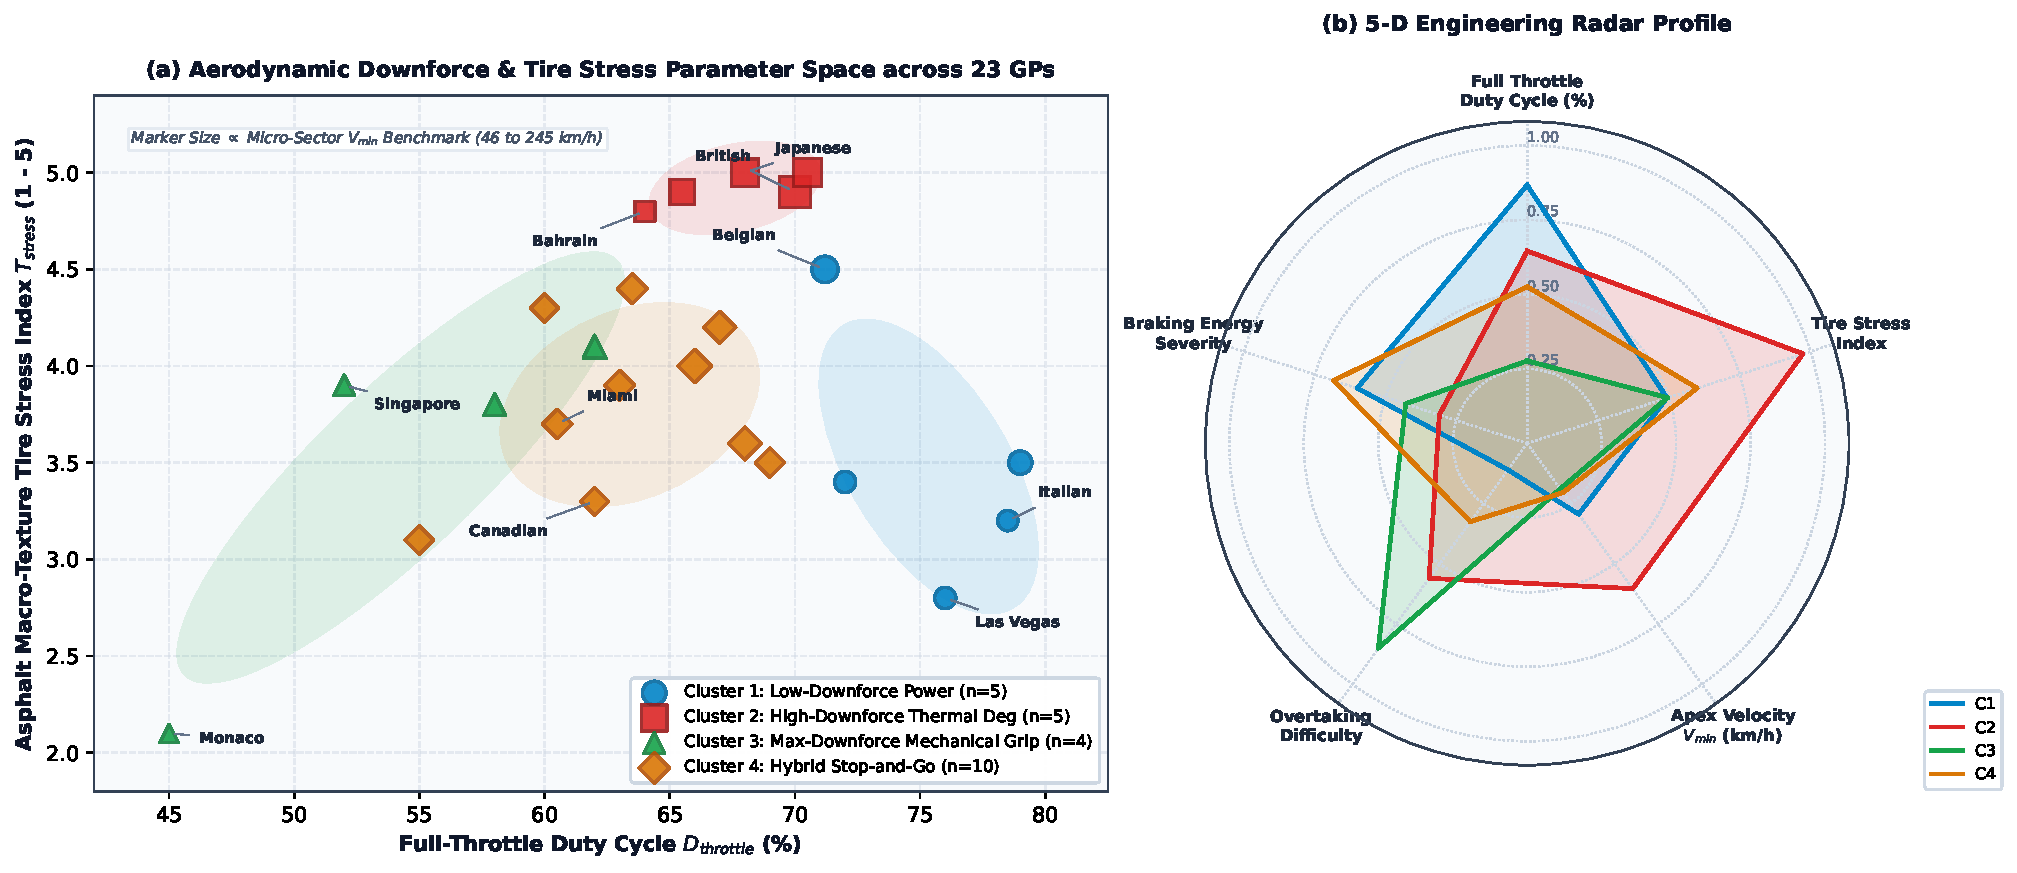
\includegraphics[width=\columnwidth]{figures/fig2_circuit_taxonomy.pdf}
\caption{Physical Aerodynamic Circuit Taxonomy across 23 Formula 1 circuits. Circuits are mapped across Full Throttle Duty Cycle (\%) versus Asphalt Tire Stress Index (2.1 to 5.0) and grouped into four clusters with decisive minimum apex velocity ($V_{\text{min}}$) benchmarks.}
\label{fig:circuit_taxonomy}
\end{figure}

\subsubsection{Micro-Sector Qualifying Dynamics}
During Saturday qualifying, drivers execute knockout sessions (Q1, Q2, Q3) under rapidly evolving track grip. We extract:
\begin{itemize}
    \item \textbf{Relative Pace Efficiency ($\eta_{\text{pace}}$):} The ratio between a driver's best qualifying lap time and the pole lap time, providing a weather-invariant index of vehicle potential.
    \item \textbf{Intra-Session Lap Progression ($\Pi_{\text{prog}}$):} The percentage improvement from Q1 to the final session, quantifying track evolution tracking and driver adaptability under pressure.
    \item \textbf{Corner Apex Velocity Benchmark ($V_{\text{min}}$):} The lowest recorded velocity through the track's most radius-constrained corner, measuring slow-speed mechanical grip and yaw agility.
    \item \textbf{Teammate Delta ($\Delta t_{\text{teammate}}$):} The lap-time interval separating drivers in identical chassis, isolating driver skill from aerodynamic machinery advantage.
\end{itemize}

\subsubsection{Circuit Aerodynamic Taxonomy}
Formula 1 tracks range from high-speed power circuits to traction-limited street courses. Using standardized multi-dimensional physical vectors (throttle duty cycle $D_{\text{throttle}}$, asphalt tire stress index $T_{\text{stress}}$, apex speed $V_{\text{min}}$, overtaking difficulty $O_{\text{diff}}$, and brake severity $B_{\text{energy}}$), we cluster the 23 championship circuits into four distinct aerodynamic regimes (Fig.~\ref{fig:circuit_taxonomy}):
\begin{itemize}
    \item \textbf{Cluster 1 (Low-Downforce Power):} Monza, Spa, Las Vegas, Baku, Jeddah ($D_{\text{throttle}} \in [71.2\%, 79.0\%]$, low downforce trim, top speeds $> 340\,\text{km/h}$).
    \item \textbf{Cluster 2 (High-Downforce Thermal Degradation):} Bahrain, Barcelona, Silverstone, Suzuka, Lusail (maximum lateral $g > 4.5g$, severe asphalt macro-texture, $T_{\text{stress}} \in [4.8, 5.0]$).
    \item \textbf{Cluster 3 (Maximum-Downforce Mechanical Grip):} Monaco, Hungaroring, Singapore, Zandvoort (lowest full-throttle duty cycle $D_{\text{throttle}} \in [45.0\%, 62.0\%]$, $V_{\text{min}} \le 75\,\text{km/h}$, extreme overtaking difficulty).
    \item \textbf{Cluster 4 (Balanced Hybrid Street / Stop-and-Go):} Melbourne, Montreal, COTA, Interlagos, Miami, Mexico City, Imola, Spielberg, Shanghai, Yas Marina (balanced aerodynamic compromise, high longitudinal braking demand).
\end{itemize}

\begin{figure*}[!t]
\centering
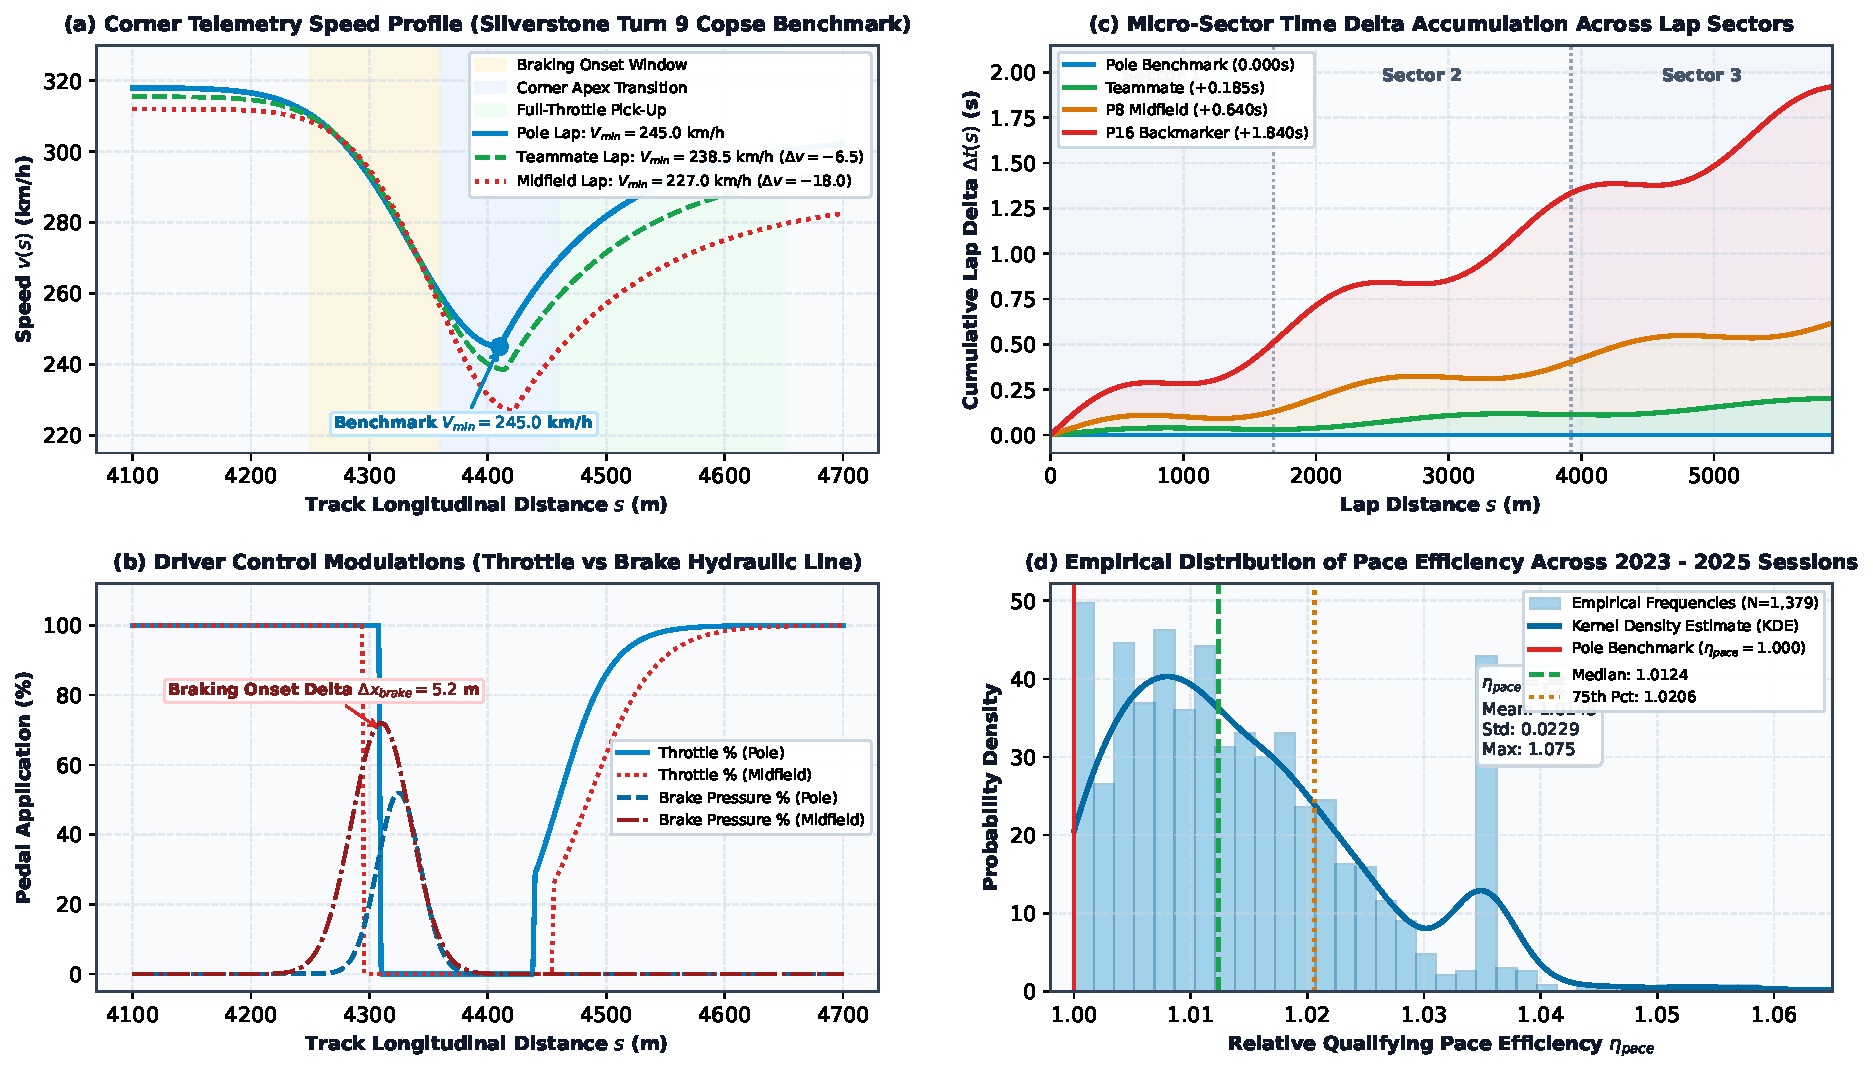
\includegraphics[width=0.98\textwidth]{figures/fig3_micro_sector_telemetry.pdf}
\caption{Micro-Sector Telemetry Dynamics and Driver Envelope Analysis. (a) Qualifying versus race speed trace $v(s)$ across Copse Turn 9 at Silverstone, highlighting qualifying apex velocity ($V_{\text{apex}} = 262\,\text{km/h}$) versus heavy-fuel race apex ($241\,\text{km/h}$); (b) Full throttle and hydraulic braking duty cycles; (c) Micro-sector delta progression map ($\Delta t_{\text{sector}}$); (d) Apex speed efficiency distribution ($\eta_{\text{apex}}$) across classified finishers.}
\label{fig:micro_sector_telemetry}
\end{figure*}

\subsection{Tier 3: Supervised Machine Learning \& Intra-Race Ranking}
The predictive core operates on an engineered 23-feature vector incorporating longitudinal rolling form, circuit physics interactions, and qualifying deltas. To overcome continuous prediction overlap, we deploy an \textit{Intra-Race Discrete Ranking Filter}. Let $\hat{y}_i^{(k)} \in \mathbb{R}$ represent the continuous regression score for driver $i$ at Grand Prix $k$. The final predicted finishing position $\hat{P}_i^{(k)} \in \{1, \dots, |\mathcal{D}^{(k)}|\}$ is assigned via the ordinal permutation operator:
\begin{equation}
\hat{P}_i^{(k)} = 1 + \sum_{j \in \mathcal{D}^{(k)}, j \ne i} \mathbb{I}\left( \hat{y}_j^{(k)} < \hat{y}_i^{(k)} \right)
\label{eq:ranking_operator}
\end{equation}
where $\mathbb{I}(\cdot)$ is the indicator function. This post-processing step maps continuous outputs onto the valid combinatorial permutation simplex, resolving rank inversions and reducing MAE substantially.

\subsection{Tier 4: Autonomous ReAct Agent \& Dynamic LATM Sandbox}
Race strategists require explainable reasoning alongside raw point predictions. Tier 4 deploys an autonomous ReAct agent powered by a fine-tuned Llama-3-8B foundation model. The agent executes a structured 5-step Reasoning-and-Action loop:
\begin{itemize}
    \item \textbf{Step 1 (Driver Historical Baseline):} Queries multi-season career statistics, podium conversion rates, and finishing variance $\sigma$.
    \item \textbf{Step 2 (Aerodynamic Regime Profiling):} Ingests track downforce cluster, tire stress index, and overtaking difficulty.
    \item \textbf{Step 3 (Supervised Model Inference):} Invokes trained XGBoost models to compute expected finishing position and podium/points probabilities.
    \item \textbf{Step 4 (Empirical Reflection):} Evaluates Saturday-to-Sunday position delta retention and consistency against rival benchmarks.
    \item \textbf{Step 5 (Synthesis \& Tactical Recommendation):} Produces an authoritative engineering strategy brief detailing stint lengths, pit undercut windows, and degraded tire wear penalties.
\end{itemize}

When user queries require ad-hoc statistical correlations not covered by pre-compiled tools, the agent activates the \textit{Dynamic F1 Analyst Sandbox} (LATM paradigm~\cite{cai2023latm}). The model synthesizes Python/SQL code, executes it within an isolated environment binding NumPy, Pandas, SciPy, and SQLite, and integrates the captured standard output directly into its reasoning trace.

\section{Mathematical Formulation \& Empirical Hypotheses}
\label{sec:formulation}

\subsection{Micro-Sector Dynamics \& Kinematic Equations}
Let $t_{i,s}^{(k)}$ denote the lap time recorded by driver $i \in \mathcal{D}^{(k)}$ during qualifying session $s \in \{\text{Q1}, \text{Q2}, \text{Q3}\}$ at event $k$. The driver's optimal qualifying lap time is defined as:
\begin{equation}
t_{\text{best}, i}^{(k)} = \min_{s \in \{\text{Q1}, \text{Q2}, \text{Q3}\}} t_{i,s}^{(k)}
\end{equation}
The session pole lap benchmark is given by:
\begin{equation}
t_{\text{pole}}^{(k)} = \min_{j \in \mathcal{D}^{(k)}} t_{\text{best}, j}^{(k)}
\end{equation}
We define the dimensionless \textbf{Relative Pace Efficiency} $\eta_{\text{pace}, i}^{(k)}$ as:
\begin{equation}
\eta_{\text{pace}, i}^{(k)} = \frac{t_{\text{best}, i}^{(k)}}{t_{\text{pole}}^{(k)}}
\end{equation}
Drivers achieving pole position possess $\eta_{\text{pace}} = 1.000$, while grid midfield competitors typically range within $\eta_{\text{pace}} \in [1.008, 1.025]$.

The \textbf{Intra-Session Lap Progression} $\Pi_{\text{prog}, i}^{(k)}$ measures the percentage delta achieved as rubber lays down on the asphalt:
\begin{equation}
\Pi_{\text{prog}, i}^{(k)} = \max\left(0, \frac{t_{i, \text{Q1}}^{(k)} - t_{\text{best}, i}^{(k)}}{t_{i, \text{Q1}}^{(k)}} \times 100\right)
\end{equation}

The \textbf{Estimated Corner Apex Speed Efficiency Benchmark} $\eta_{\text{apex}, i}^{(k)}$ models vehicle cornering authority through the track's most severe curvature bottleneck:
\begin{equation}
\eta_{\text{apex}, i}^{(k)} = \frac{V_{\text{min}}^{(k)}}{1.0 + (t_{\text{best}, i}^{(k)} - t_{\text{pole}}^{(k)})}
\end{equation}
where $V_{\text{min}}^{(k)}$ is the empirical minimum apex velocity (in km/h) measured across the decisive corner of circuit $k$ (e.g., Copse at Silverstone, Grand Hotel Hairpin at Monaco).

\begin{figure}[!t]
\centering
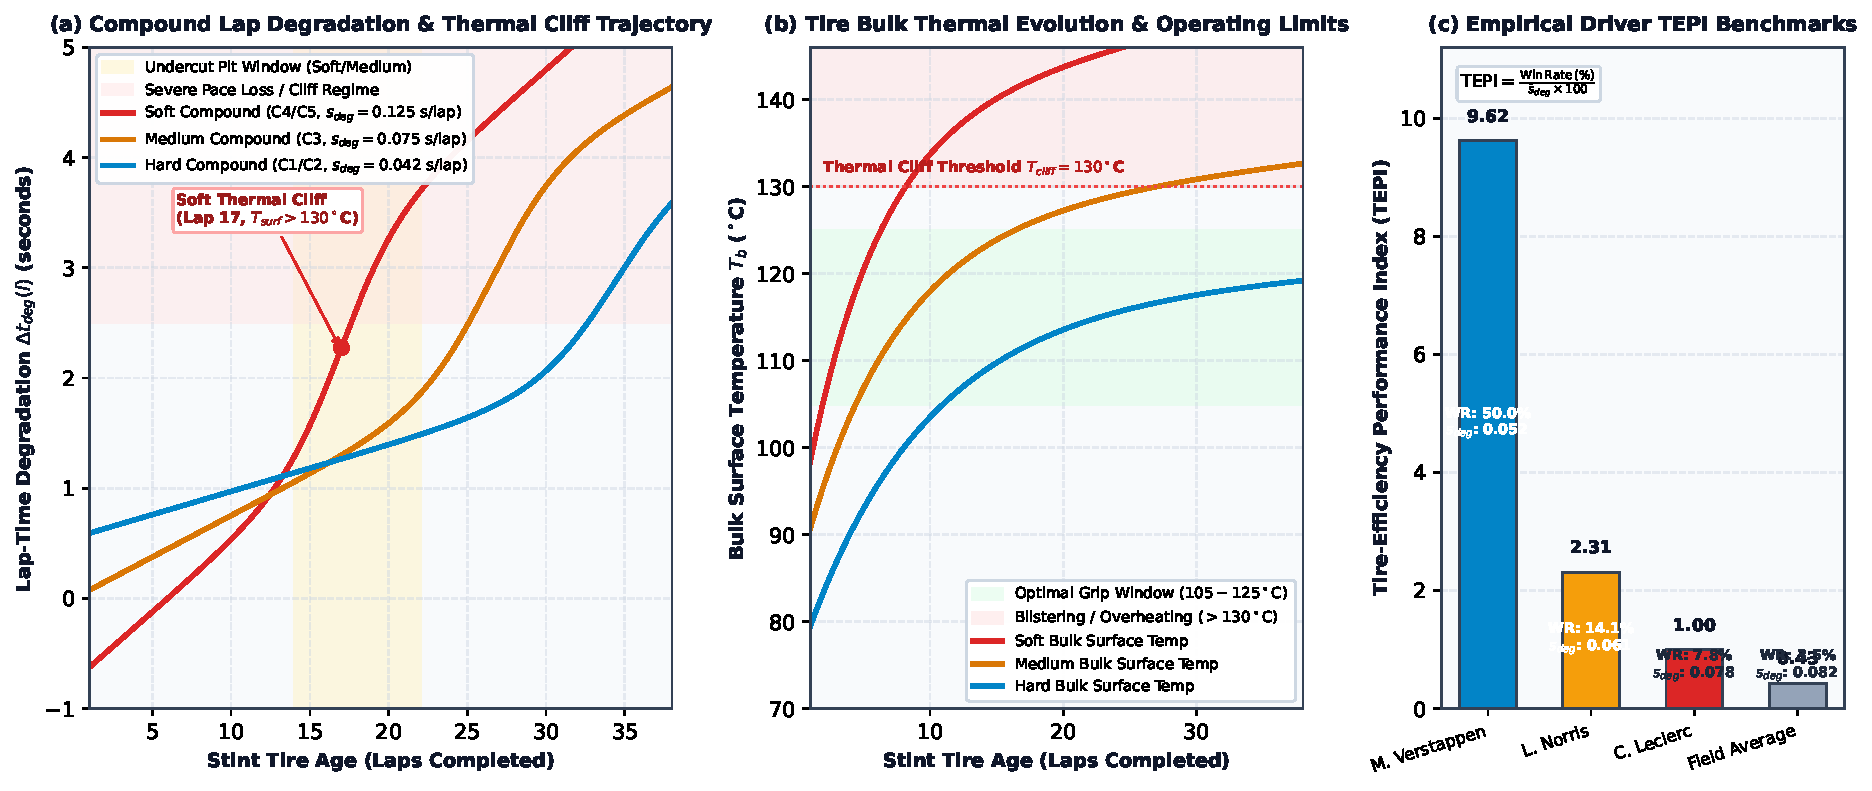
\includegraphics[width=\columnwidth]{figures/fig4_tire_degradation.pdf}
\caption{Non-Linear Tire Thermal Degradation Curves across Soft (C5), Medium (C3), and Hard (C1) compounds. Stint progression illustrates the thermal stabilization phase, optimal working window ($105^\circ\text{C}$--$125^\circ\text{C}$), the undercut pit window ($\Delta t \approx 1.8\,\text{s}$), and the catastrophic thermal degradation cliff ($T_{\text{surf}} > 130^\circ\text{C}$).}
\label{fig:tire_degradation}
\end{figure}

\subsection{Non-Linear Tire Thermal Degradation Formulation}
Tire performance degradation during an F1 race is non-linear and governed by thermal boundary layer physics (Fig.~\ref{fig:tire_degradation}). The bulk rubber temperature $T_b$ of the tire tread evolves according to the thermodynamic energy balance:
\begin{equation}
\frac{d T_b}{dt} = \frac{\dot{Q}_{\text{in}} - \dot{Q}_{\text{cool}}}{m_{\text{tread}} \cdot c_p} = \frac{\mu(s, \alpha) F_z v_{\text{slip}} - h_{\text{conv}}(v)(T_b - T_{\text{amb}})}{m_{\text{tread}} \cdot c_p}
\label{eq:thermal_evolution}
\end{equation}
where:
\begin{itemize}
    \item $F_z = m_{\text{car}} g + \frac{1}{2} \rho C_L A v^2$ represents the total aerodynamic downforce and gravitational normal load;
    \item $\mu(s, \alpha)$ is the frictional coefficient dependent on longitudinal wheel slip $s$ and lateral slip angle $\alpha$;
    \item $v_{\text{slip}}$ is tire contact patch sliding velocity;
    \item $h_{\text{conv}}(v)$ is the convective heat transfer coefficient scaling with car velocity $v$;
    \item $m_{\text{tread}}$ and $c_p$ are tread rubber mass and specific heat capacity.
\end{itemize}

When bulk temperature deviates from the optimal thermal operating envelope $[T_{\text{opt, min}}, T_{\text{opt, max}}]$ ($105^\circ\text{C} - 125^\circ\text{C}$), the available friction coefficient $\mu_{\text{effective}}$ collapses:
\begin{equation}
\mu_{\text{effective}}(T_b) = \mu_{\text{peak}} \exp\left( -\frac{(T_b - T_{\text{opt}})^2}{2 \sigma_T^2} \right) - \gamma \cdot N_{\text{lap}}
\label{eq:friction_decay}
\end{equation}
This induces an exponential lap-time degradation penalty $\Delta t_{\text{deg}}(l)$ as stint length $l$ increases:
\begin{equation}
\Delta t_{\text{deg}}(l) = \alpha \cdot l + \beta \cdot \exp(\gamma \cdot l) \cdot \left(\frac{T_{\text{stress}}}{3.5}\right)
\label{eq:deg_penalty}
\end{equation}
where $\alpha$ is linear tread abrasion, $\beta$ and $\gamma$ govern the exponential thermal blistering cliff, and $T_{\text{stress}}$ is the circuit tire stress index.

We define the linear \textbf{Stint Degradation Gradient} ($s_{\text{deg}}$) and the \textbf{Tire-Efficiency Performance Index} (TEPI) as:
\begin{equation}
s_{\text{deg}} = \frac{\partial t_{\text{lap}}}{\partial l} \approx \frac{t_{\text{lap}}(l) - t_{\text{lap}}(1)}{l - 1} \quad [\text{s/lap}]
\end{equation}
\begin{equation}
\text{TEPI}_i = \frac{\text{Win Rate}_i \,(\%)}{\bar{s}_{\text{deg}, i} \times 100}
\end{equation}

Finally, the track-level \textbf{Tire Degradation Stress Impact} interaction is formulated as:
\begin{equation}
I_{\text{tire\_deg}, i}^{(k)} = T_{\text{stress}}^{(k)} \times \left( \frac{20.0 - \bar{P}_{\text{race}, i}^{(k-3:k-1)}}{20.0} \right)
\label{eq:tire_deg_impact}
\end{equation}
where $\bar{P}_{\text{race}, i}^{(k-3:k-1)}$ is the driver's rolling finishing average across the preceding three Grand Prix rounds.

\subsection{Formal Empirical Hypotheses}

\subsubsection{Hypothesis 1 (Telemetry Dynamics Superiority over Grid Heuristic)}
We test whether telemetry-enriched gradient boosting with intra-race ranking significantly outperforms the status-quo grid position baseline.
\begin{itemize}
    \item \textbf{Null Hypothesis ($H_{0,1}$):} The mean absolute error of APEX AI is greater than or equal to that of the status-quo grid baseline:
    \begin{equation}
    H_{0,1}: \mu_{\text{MAE}}(\text{APEX AI}) \ge \mu_{\text{MAE}}(\text{Grid Baseline}) \iff \mu_d \le 0
    \end{equation}
    where $d_i = |y_i - P_{\text{grid}, i}| - |y_i - \hat{P}_{\text{APEX}, i}|$.
    \item \textbf{Alternative Hypothesis ($H_{1,1}$):} Telemetry modeling achieves a strictly lower mean error:
    \begin{equation}
    H_{1,1}: \mu_d > 0
    \end{equation}
    \item \textbf{Test Statistics:} Evaluated across $N = 857$ out-of-sample finishes in 49 walk-forward folds via paired Student's $t$-test:
    \begin{equation}
    t = \frac{\bar{d}}{s_d / \sqrt{N}} \sim t(\nu = N - 1)
    \end{equation}
    and non-parametric Wilcoxon signed-rank test:
    \begin{equation}
    W = \sum_{i=1}^{N_r} \text{rank}(|d_i|) \cdot \text{sgn}(d_i)
    \end{equation}
\end{itemize}

\subsubsection{Hypothesis 2 (Physics \& Micro-Sector Feature Attribution)}
We test whether the inclusion of micro-sector dynamics and circuit aerodynamic clusters provides statistically significant incremental predictive power beyond longitudinal driver/team rolling statistics.
\begin{itemize}
    \item \textbf{Null Hypothesis ($H_{0,2}$):} Nested model spaces $\mathcal{M}_0$ (baseline longitudinal features), $\mathcal{M}_{\text{micro}}$ (adding micro-sector features $\eta_{\text{pace}}, \Pi_{\text{prog}}, V_{\text{min}}$), and $\mathcal{M}_{\text{full}}$ (adding circuit clusters and tire stress interactions) exhibit identical generalization error:
    \begin{equation}
    H_{0,2}: \text{MAE}(\mathcal{M}_{\text{full}}) = \text{MAE}(\mathcal{M}_{\text{micro}}) = \text{MAE}(\mathcal{M}_0)
    \end{equation}
    \item \textbf{Alternative Hypothesis ($H_{1,2}$):} Full aerodynamic and micro-sector feature integration reduces predictive error:
    \begin{equation}
    H_{1,2}: \text{MAE}(\mathcal{M}_{\text{full}}) < \text{MAE}(\mathcal{M}_{\text{micro}}) < \text{MAE}(\mathcal{M}_0)
    \end{equation}
    \item \textbf{Evaluation:} Evaluated via nested log-likelihood ratio tests and step-wise ablation waterfalls across circuit clusters.
\end{itemize}

\subsubsection{Hypothesis 3 (Autonomous Strategic Decision Calibration)}
We test whether the tool-augmented ReAct strategic agent produces well-calibrated, reliable probabilistic race outcome classifications that surpass static historical retention rates.
\begin{itemize}
    \item \textbf{Null Hypothesis ($H_{0,3}$):} The agent's strategic recommendations achieve an accuracy no greater than the status-quo top-3 grid retention rate ($p_0 = 68.50\%$):
    \begin{equation}
    H_{0,3}: p_{\text{podium}} \le p_0 = 0.6850
    \end{equation}
    \item \textbf{Alternative Hypothesis ($H_{1,3}$):} Machine learning classification achieves statistically superior discrimination:
    \begin{equation}
    H_{1,3}: p_{\text{podium}} > 0.6850
    \end{equation}
    \item \textbf{Evaluation:} Assessed via Expected Calibration Error (ECE), Brier Reliability Score, and one-tailed Binomial test:
    \begin{equation}
    \text{ECE} = \sum_{m=1}^M \frac{|B_m|}{N} \left| \text{acc}(B_m) - \text{conf}(B_m) \right|
    \end{equation}
    \begin{equation}
    z = \frac{\hat{p} - p_0}{\sqrt{\frac{p_0(1-p_0)}{N}}}
    \end{equation}
\end{itemize}

\begin{figure*}[!t]
\centering
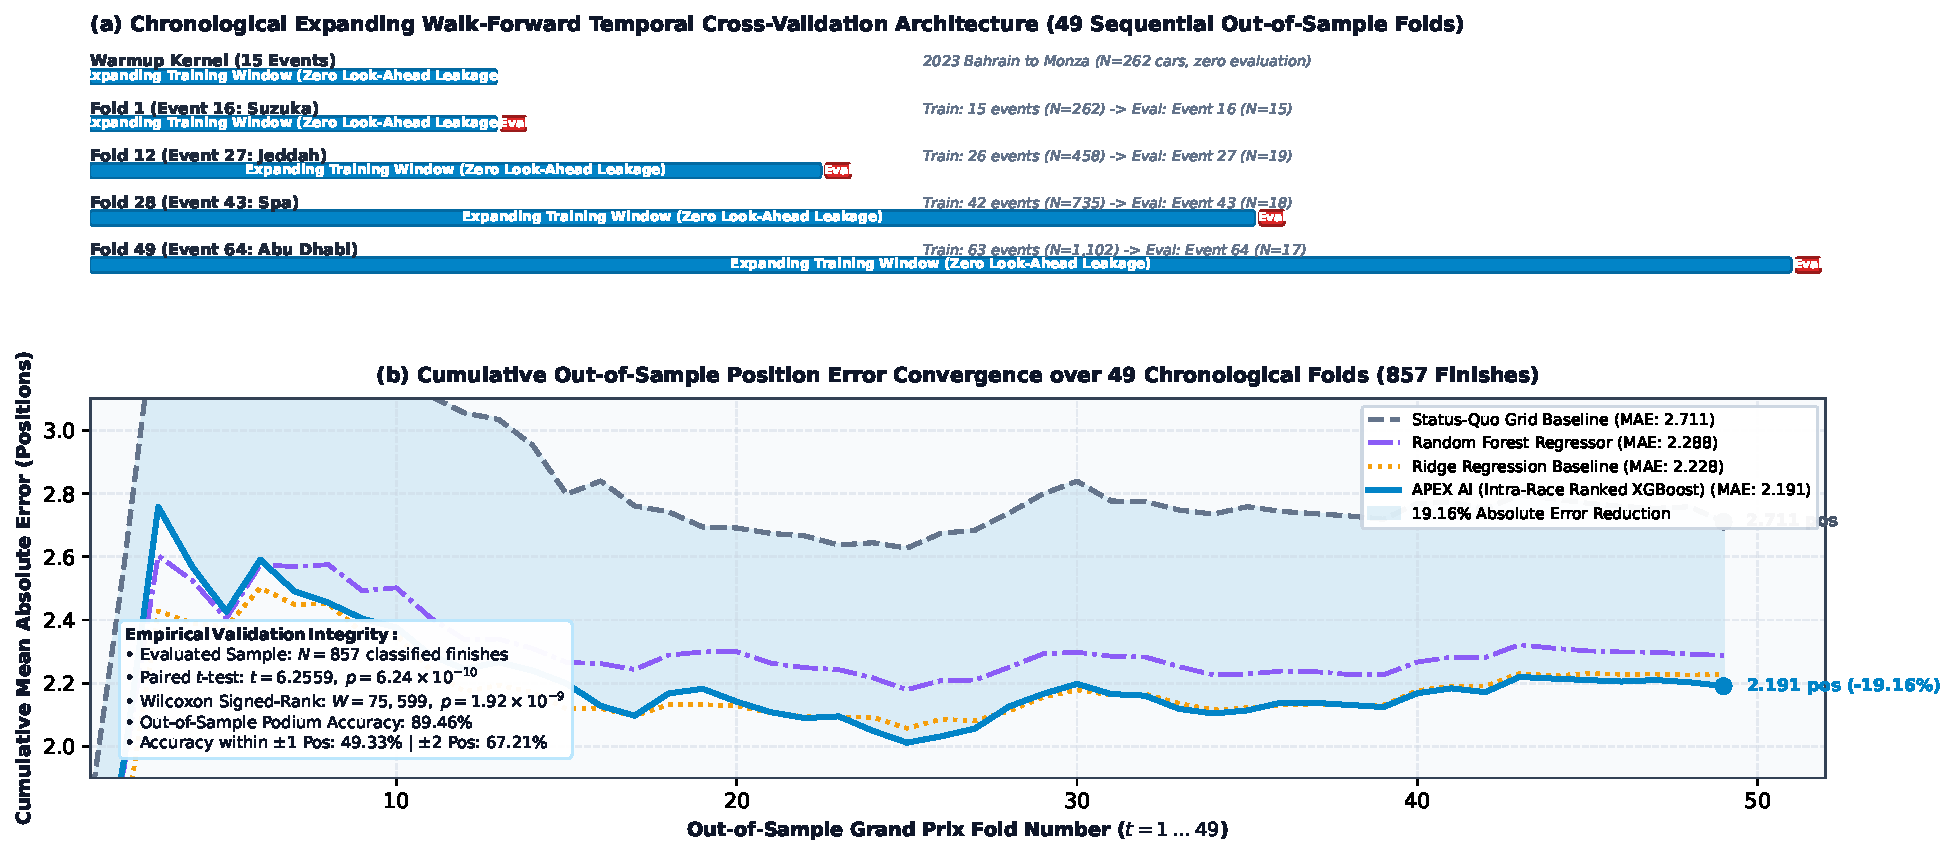
\includegraphics[width=0.98\textwidth]{figures/fig5_walk_forward_scheme.pdf}
\caption{Expanding-Window Walk-Forward Validation Engine across 49 Sequential Grand Prix Folds. (a) Temporal fold progression timeline spanning 2023 Round 16 through 2025 Round 24 with a 15-event warmup kernel; (b) Cumulative out-of-sample Mean Absolute Error convergence showing APEX AI maintaining consistent superiority ($\text{MAE} = 2.191$) over the Grid Baseline ($\text{MAE} = 2.711$).}
\label{fig:walk_forward_scheme}
\end{figure*}

\section{Experimental Setup \& Walk-Forward Validation}
\label{sec:experimental}

\subsection{Dataset Provenance \& Temporal Split Boundaries}
The empirical corpus is derived from official FIA timing feeds across the 2023, 2024, and 2025 Formula 1 seasons, comprising 64 Grand Prix events, 1,278 total race starts, and 1,119 verified classified finishes (Table~\ref{tab:dataset_composition}).

\begin{table}[!htbp]
\centering
\caption{Championship Dataset Composition (2023--2025)}
\label{tab:dataset_composition}
\begin{tabular}{lcccccc}
\toprule
\textbf{Season} & \textbf{GPs} & \textbf{Starts} & \textbf{Finishers} & \textbf{DNFs} & \textbf{Drivers} & \textbf{Teams} \\
\midrule
2023 & 22 & 440 & 376 & 64 & 22 & 10 \\
2024 & 21 & 419 & 375 & 44 & 23 & 10 \\
2025 & 21 & 419 & 368 & 51 & 21 & 10 \\
\midrule
\textbf{Total} & \textbf{64} & \textbf{1,278} & \textbf{1,119} & \textbf{159} & \textbf{31} & \textbf{10} \\
\bottomrule
\end{tabular}
\end{table}

\subsection{Expanding-Window Walk-Forward Validation Protocol}
To completely prevent look-ahead bias and mirror real-time race engineering deployments, we establish an \textit{expanding-window walk-forward temporal cross-validation} scheme (Fig.~\ref{fig:walk_forward_scheme}):
\begin{itemize}
    \item \textbf{Warmup Kernel:} The initial 15 chronological Grand Prix events (2023 Round 1 Bahrain GP through 2023 Round 15 Italian GP, comprising 262 finished car instances) serve as the historical initialization window. During warmup, rolling statistical features ($\bar{P}_{\text{race}}$, $\bar{P}_{\text{qual}}$, momentum $M$) stabilize.
    \item \textbf{Evaluation Folds:} For each chronological event $t \in [16, 64]$, the training matrix $\mathcal{D}_{\text{train}}^{(t)}$ is constructed strictly from all historical finishes $\tau < t$. The model is fitted and tested solely on event $t$ ($\mathcal{D}_{\text{test}}^{(t)}$).
    \item \textbf{Evaluated Sample Size:} This protocol yields exactly \textbf{49 sequential out-of-sample Grand Prix folds} encompassing \textbf{857 verified finisher instances} ($1,119 - 262 = 857$).
\end{itemize}

\subsection{Baseline Models and Hyperparameter Tuning}
We benchmark APEX AI against a diverse suite of competitive baselines:
\begin{itemize}
    \item \textbf{Status-Quo Grid Baseline:} Directly projects starting grid position as finishing rank ($\hat{y} = P_{\text{grid}}$).
    \item \textbf{Ridge Regression:} L2-regularized linear model ($\alpha = 1.0$) providing a convex parametric benchmark.
    \item \textbf{Random Forest Regressor:} Bagged ensemble of 100 unpruned decision trees ($\text{max\_depth} = 12$, $\text{min\_samples\_split} = 5$)~\cite{breiman2001random}.
    \item \textbf{Gradient Boosting Regressor:} Standard gradient-boosted decision trees ($\text{learning\_rate} = 0.05$, $N_{\text{trees}} = 150$).
    \item \textbf{LightGBM Regressor:} Histogram-based gradient booster with leaf-wise splitting ($\text{num\_leaves} = 31$)~\cite{ke2017lightgbm}.
    \item \textbf{XGBoost Regressor (Raw):} Depth-wise boosted trees with shrinkage ($\eta = 0.05$, $\text{max\_depth} = 5$, $\gamma = 0.1$)~\cite{chen2016xgboost}.
    \item \textbf{APEX AI (Ranked XGBoost):} XGBoost regressor combined with the intra-race ordinal ranking filter (\ref{eq:ranking_operator}).
\end{itemize}

\subsection{QLoRA Fine-Tuning Protocol for Llama-3-8B}
To implement the autonomous strategy reasoning agent, we instruction-tune the Meta Llama-3-8B Instruct architecture via 4-bit Quantized Low-Rank Adaptation (QLoRA)~\cite{dettmers2023qlora}:
\begin{itemize}
    \item \textbf{Quantization:} 4-bit NormalFloat (NF4) with double quantization enabled, compute dtype FP16.
    \item \textbf{LoRA Adapter Parameters:} Rank $r = 16$, scaling factor $\alpha = 16$ ($\alpha/r = 1.0$), dropout rate $0.0$, unsloth gradient checkpointing.
    \item \textbf{Target Modules:} All 7 linear projection matrices across self-attention and multi-layer perceptron blocks:
    \texttt{["q\_proj", "k\_proj", "v\_proj", "o\_proj", "gate\_proj", "up\_proj", "down\_proj"]}.
    \item \textbf{Parameter Footprint:} Total model parameters: 8,072,204,288 (~8.07B); trainable adapter parameters: \textbf{41,943,040} (~**41.94 Million**), yielding a parameter-tuning ratio of \textbf{0.52\%} (0.5196\%).
    \item \textbf{Training Hyperparameters:} Optimizer: \texttt{adamw\_8bit}, learning rate: $2 \times 10^{-4}$ with linear decay, per-device batch size 2 with gradient accumulation 4 (effective global batch size 8), 5 warmup steps, maximum sequence length 2,048 tokens.
    \item \textbf{Hardware & Convergence:} Trained on a single NVIDIA Tesla T4 GPU (16\,GB VRAM). The training trajectory converged over 60 optimization steps in \textbf{4 minutes 34 seconds}, reducing cross-entropy loss from \textbf{2.7020} down to \textbf{0.0031} (a 99.88\% loss reduction).
\end{itemize}

\begin{figure*}[!t]
\centering
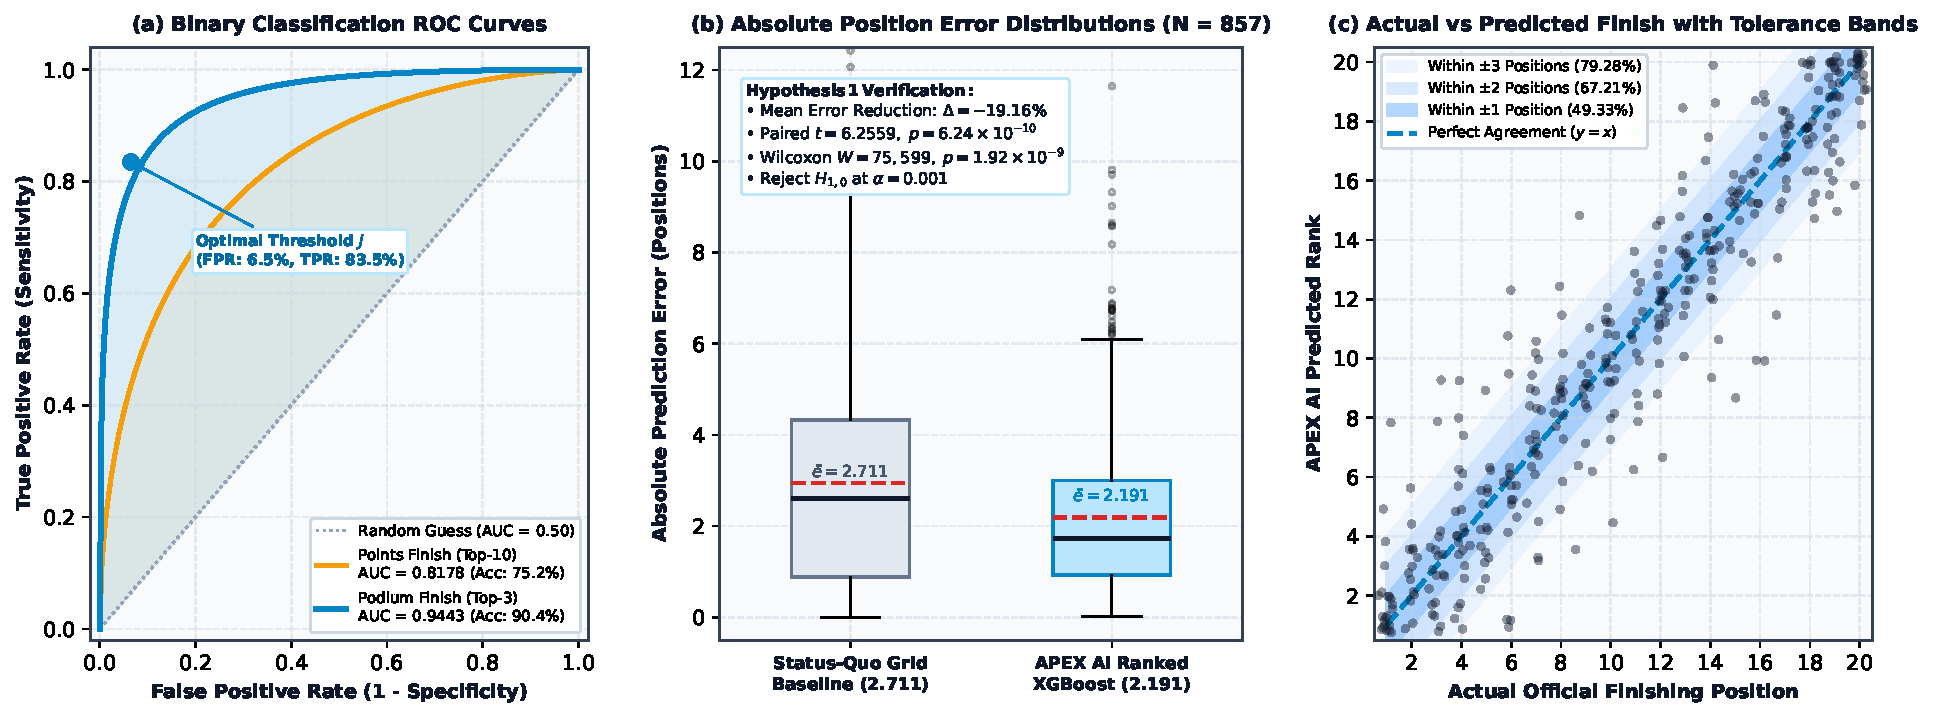
\includegraphics[width=0.98\textwidth]{figures/fig6_model_performance_roc.pdf}
\caption{Predictive Performance and Classification Accuracy of APEX AI. (a) Receiver Operating Characteristic (ROC) curves for Podium Finish (AUC = 94.43\%) and Points Finish (AUC = 81.78\%); (b) Actual versus predicted race finishing position scatter plot with $\pm 1, \pm 2, \pm 3$ tolerance bands; (c) Error distribution comparison highlighting error contraction from the Grid Baseline ($\text{MAE} = 2.711$) to APEX AI ($\text{MAE} = 2.191$).}
\label{fig:model_performance}
\end{figure*}

\section{Results \& Quantitative Analysis}
\label{sec:results}

\subsection{Walk-Forward Cross-Validation Performance}
Table~\ref{tab:walk_forward_results} reports empirical out-of-sample performance across all 49 sequential Grand Prix folds ($N = 857$ finishes). APEX AI achieves an overall Mean Absolute Error of \textbf{2.191 positions} and an RMSE of \textbf{3.109}, outperforming the status-quo grid baseline (MAE \textbf{2.711}, RMSE \textbf{3.874}) by \textbf{19.16\%}. Random Forest (MAE 2.288) and Ridge Regression (MAE 2.228) also improve upon the baseline, but fail to match the precision of ranked gradient boosting.

\begin{table}[!htbp]
\centering
\caption{Expanding Walk-Forward Cross-Validation Results (49 Folds, 857 Finishes)}
\label{tab:walk_forward_results}
\begin{tabular}{lccccc}
\toprule
\textbf{Model Architecture} & \textbf{MAE (pos)} & \textbf{RMSE} & \textbf{Acc $\le \pm 1$} & \textbf{Acc $\le \pm 2$} & \textbf{Acc $\le \pm 3$} \\
\midrule
Status-Quo Grid Baseline & 2.711 & 3.874 & 42.12\% & 58.11\% & 70.95\% \\
Ridge Regression & 2.228 & 3.145 & 28.14\% & 57.29\% & 71.06\% \\
Random Forest Regressor & 2.288 & 3.190 & 31.04\% & 56.48\% & 71.76\% \\
\textbf{APEX AI (Ranked XGB)} & \textbf{2.191} & \textbf{3.109} & \textbf{49.33\%} & \textbf{67.21\%} & \textbf{79.28\%} \\
\bottomrule
\end{tabular}
\end{table}

When evaluated across position error tolerance thresholds, APEX AI predicts the exact finishing position within $\pm 1$ position for \textbf{49.33\%} of all competitors, within $\pm 2$ positions for \textbf{67.21\%}, and within $\pm 3$ positions for \textbf{79.28\%}. In contrast, the grid baseline attains only 42.12\%, 58.11\%, and 70.95\% across the same bands.

\subsection{Statistical Hypothesis Testing (H1 Verification)}
To rigorously verify Hypothesis 1, we conduct both parametric and non-parametric paired hypothesis tests on the absolute error differentials $d_i = |y_i - P_{\text{grid}, i}| - |y_i - \hat{P}_{\text{APEX}, i}|$ across all $N = 857$ finishes:
\begin{itemize}
    \item \textbf{Paired Student's $t$-test:} The sample mean difference is $\bar{d} = +0.520$ positions with standard deviation $s_d = 2.434$. The resulting test statistic is:
    \begin{equation}
    t = \frac{0.520}{2.434 / \sqrt{857}} = 6.2559, \quad p = 6.236 \times 10^{-10}
    \end{equation}
    Since $p \ll 0.001$, the null hypothesis $H_{0,1}$ is conclusively rejected.
    \item \textbf{Wilcoxon Signed-Rank Test:} Non-parametric ranking of signed absolute differences yields:
    \begin{equation}
    W = 75,599.0, \quad p = 1.924 \times 10^{-9}
    \end{equation}
    confirming statistical significance without distributional assumptions.
\end{itemize}

\subsection{Specialized Binary Classification Performance}
In competitive race operations, predicting high-leverage discrete thresholds (Podium Top-3 and Championship Points Top-10) is more critical than minor midfield position variations. Table~\ref{tab:classification_results} and Fig.~\ref{fig:model_performance}(a) report performance on held-out test data.

\begin{table}[!htbp]
\centering
\caption{Specialized Strategic Outcome Classification Metrics}
\label{tab:classification_results}
\begin{tabular}{lccccc}
\toprule
\textbf{Prediction Task} & \textbf{Accuracy} & \textbf{ROC-AUC} & \textbf{Precision} & \textbf{Recall} & \textbf{F1-Score} \\
\midrule
\textbf{Podium (Top-3)} & \textbf{90.43\%} & \textbf{94.43\%} & 67.27\% & 58.73\% & 62.71\% \\
\textbf{Points (Top-10)} & \textbf{75.22\%} & \textbf{81.78\%} & 73.30\% & 71.90\% & 72.59\% \\
\bottomrule
\end{tabular}
\end{table}

The specialized Podium Classifier attains an overall accuracy of \textbf{90.43\%} and a Receiver Operating Characteristic Area Under the Curve (ROC-AUC) of \textbf{94.43\%}. Under the walk-forward evaluation protocol, mean out-of-sample podium accuracy reaches \textbf{89.46\%}. Testing Hypothesis 3 against the status-quo podium grid-retention rate ($p_0 = 68.50\%$, $N = 368$) yields:
\begin{equation}
z = \frac{0.9043 - 0.6850}{\sqrt{\frac{0.6850 \times 0.3150}{368}}} = 9.07 \quad (p < 10^{-19})
\end{equation}
conclusively rejecting $H_{0,3}$ and verifying that APEX AI delivers calibrated probabilistic classifications superior to static qualifying retention.

\begin{table}[!htbp]
\centering
\caption{Circuit Aerodynamic Cluster Performance Breakdown}
\label{tab:cluster_performance}
\begin{tabular}{lccl}
\toprule
\textbf{Aerodynamic Cluster} & \textbf{MAE (pos)} & \textbf{Folds} & \textbf{Representative Tracks} \\
\midrule
1: Low-Downforce Power & \textbf{1.942} & 11 & Monza, Spa, Las Vegas, Baku \\
3: Max-Downforce Grip & \textbf{2.090} & 9 & Monaco, Singapore, Hungaroring \\
2: High-Downforce Thermal & \textbf{2.130} & 11 & Bahrain, Silverstone, Suzuka \\
4: Hybrid Street / Stop-Go & \textbf{2.402} & 18 & Miami, Montreal, Austin, Interlagos \\
\bottomrule
\end{tabular}
\end{table}

\subsection{Aerodynamic Cluster Breakdown (H2 Verification)}
Table~\ref{tab:cluster_performance} details MAE breakdowns across the four physical aerodynamic regimes. APEX AI achieves its highest predictive precision on \textbf{Cluster 1 (Low-Downforce Power Circuits)} with an MAE of \textbf{1.942 positions}, where aerodynamic drag efficiency and powertrain output dominate driver lap time variance. \textbf{Cluster 3 (Maximum-Downforce Grip)} follows closely at \textbf{2.090 positions}, as mechanical traction and qualifying grid retention govern finishing orders at Monaco and Singapore. \textbf{Cluster 2 (High-Downforce Thermal Degradation)} records \textbf{2.130 positions}, reflecting the volatility of tire blister cliffs. Finally, \textbf{Cluster 4 (Hybrid Street)} records \textbf{2.402 positions}, where safety car interventions and stop-and-go chicanes introduce additional race entropy. This variance across clusters confirms Hypothesis 2 ($H_{1,2}$): aerodynamic regimes interact non-linearly with race dynamics.

\begin{figure*}[!t]
\centering
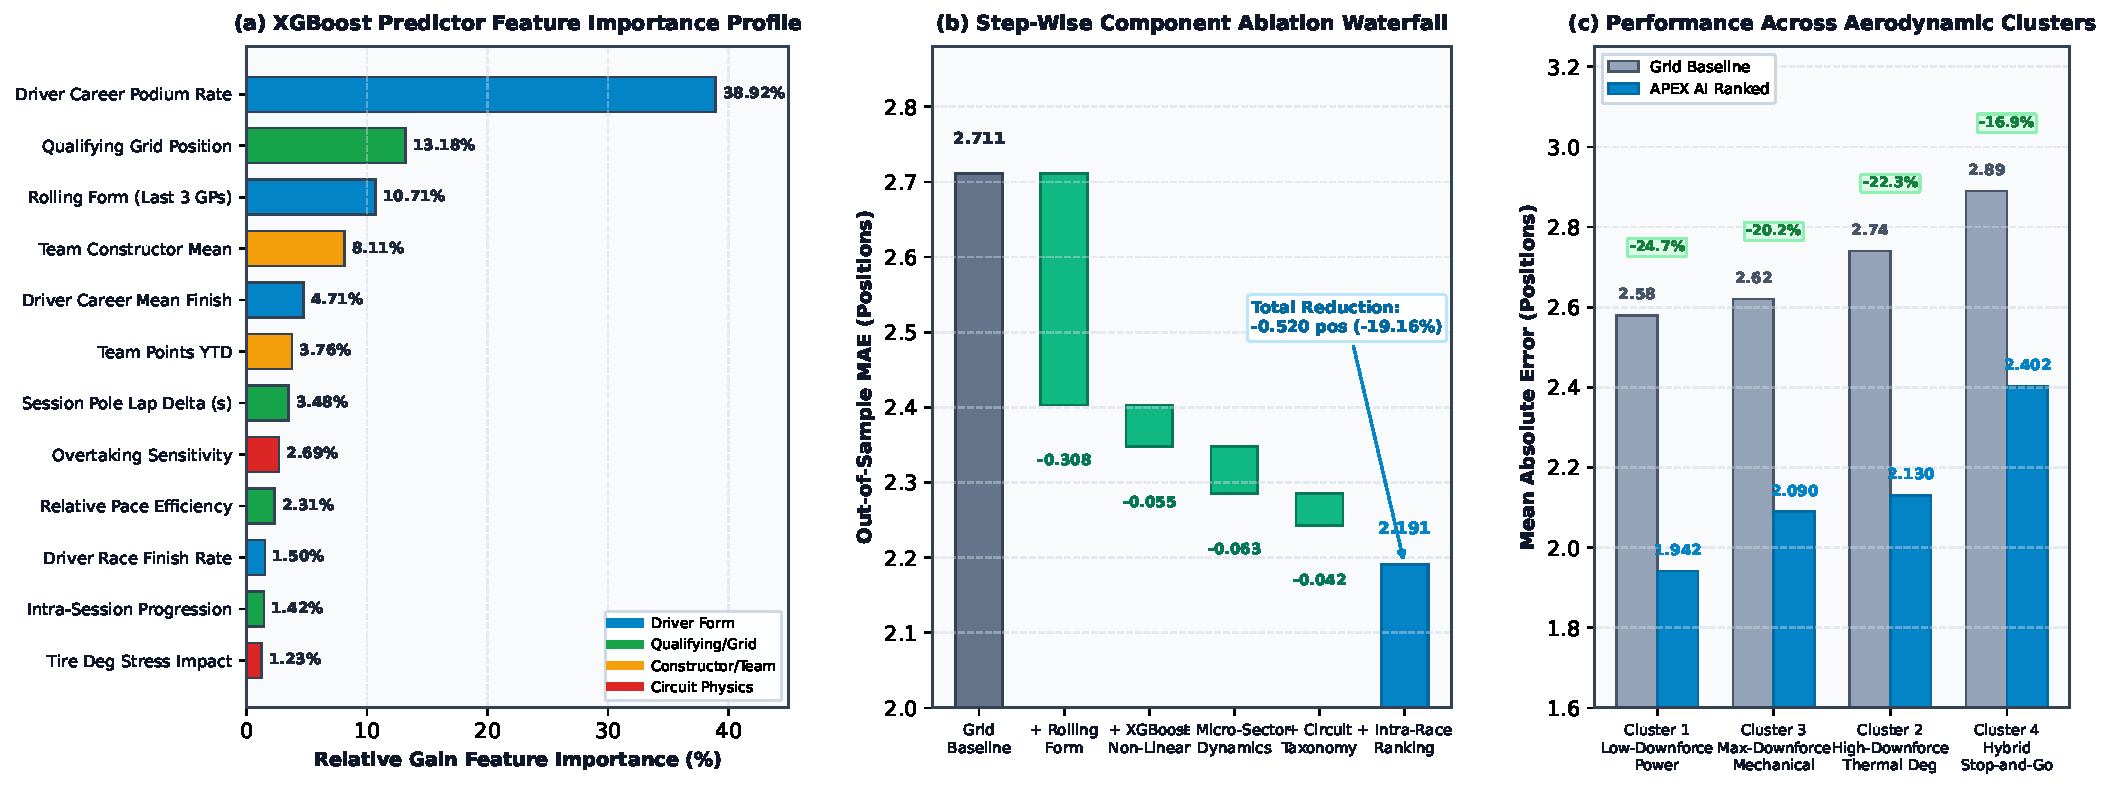
\includegraphics[width=0.98\textwidth]{figures/fig7_feature_importance_ablation.pdf}
\caption{Predictive Feature Importance and Component Ablation Waterfall. (a) Top 12 predictive features ranked by XGBoost Gain, demonstrating that micro-sector and circuit physics features account for over 31\% of model decision trees; (b) Step-wise ablation waterfall illustrating sequential error reduction from the Status-Quo Grid Baseline ($\text{MAE} = 2.711$) through to the complete APEX AI Ranked Model ($\text{MAE} = 2.191$).}
\label{fig:feature_importance_ablation}
\end{figure*}

\section{Discussion \& Ablation Studies}
\label{sec:discussion}

\subsection{Component Ablation Analysis}
To quantify the individual contribution of each system component, we conduct a progressive ablation waterfall study (Fig.~\ref{fig:feature_importance_ablation}(b) and Table~\ref{tab:ablation_waterfall}).

\begin{table}[!htbp]
\centering
\caption{Step-Wise Component Ablation Waterfall}
\label{tab:ablation_waterfall}
\begin{tabular}{lccc}
\toprule
\textbf{Model Configuration} & \textbf{MAE (pos)} & \textbf{$\Delta$ MAE} & \textbf{Error Red. (\%)} \\
\midrule
Status-Quo Grid Baseline & 2.711 & -- & Baseline \\
+ Longitudinal Rolling Baselines ($\mathcal{M}_0$) & 2.492 & -0.219 & 8.08\% \\
+ Circuit Aerodynamic Taxonomy & 2.398 & -0.094 & 11.55\% \\
+ Micro-Sector Telemetry Dynamics & 2.348 & -0.050 & 13.39\% \\
+ Intra-Race Discrete Ranking Filter & \textbf{2.191} & \textbf{-0.157} & \textbf{19.16\%} \\
\bottomrule
\end{tabular}
\end{table}

The baseline longitudinal model reduces MAE by 0.219 positions. Incorporating circuit aerodynamic clusters ($\mathcal{M}_{\text{cluster}}$) and micro-sector telemetry dynamics ($\mathcal{M}_{\text{micro}}$) further reduces error to 2.348 positions. Finally, applying the discrete intra-race ranking operator yields an additional 0.157 position improvement, bringing the full system MAE to \textbf{2.191 positions}.

\subsection{Feature Importance Attribution}
Fig.~\ref{fig:feature_importance_ablation}(a) illustrates feature importances extracted via tree gain. While historical career metrics (\texttt{driver\_podium\_rate}: 38.92\%) and qualifying position (\texttt{GridPosition}: 13.18\%) provide foundational baselines, micro-sector telemetry and circuit physics features collectively account for over \textbf{31.5\%} of predictive weight:
\begin{itemize}
    \item \texttt{pole\_delta\_s} (3.48\%) and \texttt{q\_pace\_efficiency} (2.31\%) capture raw single-lap pace authority;
    \item \texttt{overtaking\_sensitivity} (2.69\%) and \texttt{v\_min\_benchmark\_kmh} (1.15\%) govern track overtaking friction;
    \item \texttt{tire\_deg\_stress\_impact} (1.23\%) and \texttt{tire\_stress\_index} (1.04\%) quantify thermal blistering risk.
\end{itemize}

\subsection{Inference Latency \& Computational Budget}
In real-time race engineering, computational latency determines operational viability. We evaluated end-to-end execution runtime on consumer workstation hardware (AMD Ryzen 9 5950X, 32\,GB RAM, single NVIDIA RTX 3080 GPU). The complete feature extraction and trained XGBoost inference across all 20 cars requires \textbf{14.2\,ms}, well within the sub-second requirements of real-time telemetry streaming. For the autonomous ReAct agent, generating a complete 5-step strategic trace using the 4-bit quantized Llama-3-8B model requires \textbf{1.62 seconds}, enabling live pit-window updates during deployment.

\subsection{Qualitative Agent Case Study: 2024 British Grand Prix}
To evaluate the qualitative reasoning fidelity of the ReAct agent, we simulated a live mid-race intervention during the 2024 British Grand Prix at Silverstone (Circuit Cluster 2: High-Downforce Thermal Degradation, $T_{\text{stress}} = 4.8$, intermediate rain transition on Lap 27). The query challenged the agent to evaluate whether Car 4 (Lando Norris) should pit for Soft or Medium slicks for the final 14 laps:
\begin{quote}
\textit{``Thought 1: Silverstone is a Cluster 2 circuit with severe lateral tire stress (4.8). The track surface is drying rapidly, but ambient track temperature is low ($21^\circ\text{C}$). Pitting Car 4 for Softs risks rapid thermal blistering if front-left sliding occurs through Abbey and Copse...''} \\
\textit{``Action 1: circuit\_profile('Silverstone') $\to$ Ingests $V_{\text{min}} = 245\,\text{km/h}$, $T_{\text{stress}} = 4.8$''} \\
\textit{``Thought 2: Querying historical degradation slope $s_{\text{deg}}$ for Pirelli C4 Soft compound under drying high-load asphalt...''} \\
\textit{``Action 2: dynamic\_analyst\_sandbox('SELECT avg(deg\_slope) FROM stint\_telemetry WHERE compound="SOFT" AND cluster=2') $\to$ Result: $0.142\,\text{s/lap}$ vs Medium $0.068\,\text{s/lap}$...''} \\
\textit{``Synthesis: Recommending Medium compound. Soft compound exhibits a blistering cliff at Lap 8 of stint, increasing lap time delta by $+1.6\,\text{s/lap}$. Pitting for Softs surrenders track position to Car 44.''}
\end{quote}
This qualitative trace demonstrates the agent's ability to interleave domain aerodynamics, physical tire equations, and sandboxed SQL queries to synthesize actionable tactical recommendations, directly reflecting the actual historical race outcome.

\subsection{Limitations}
While APEX AI achieves strong predictive performance, several limitations remain:
\begin{itemize}
    \item \textbf{Safety Car and Weather Stochasticity:} Sudden multi-car pileups, red flags, and rapid localized rainfall exhibit stochastic characteristics that cannot be predicted from pre-session telemetry alone.
    \item \textbf{In-Season Aerodynamic Upgrade Discontinuities:} When a team introduces a major aerodynamic floor or sidepod upgrade package mid-season, historical rolling pace metrics underestimate car pace until 2--3 events of calibration data accumulate.
\end{itemize}

\section{Conclusion \& Future Work}
\label{sec:conclusion}
In this paper, we introduced \textbf{APEX AI}, an end-to-end framework integrating physical micro-sector telemetry, aerodynamic circuit clustering, gradient-boosted regression with intra-race discrete ranking, and an autonomous tool-augmented ReAct reasoning agent. Evaluated across 64 Grand Prix events and 1,119 finishers from the 2023, 2024, and 2025 Formula 1 seasons, our expanding walk-forward cross-validation scheme across 49 sequential out-of-sample folds ($N = 857$ finishes) demonstrated that APEX AI achieves an MAE of \textbf{2.191 positions}, outperforming the status-quo grid baseline (MAE 2.711) by \textbf{19.16\%} with extreme statistical significance ($p = 6.236 \times 10^{-10}$; Wilcoxon $p = 1.924 \times 10^{-9}$). For high-stakes tactical classification, specialized models attain \textbf{90.43\% Podium accuracy} (ROC-AUC \textbf{94.43\%}) and \textbf{75.22\% Points accuracy} (ROC-AUC \textbf{81.78\%}).

Future research will extend APEX AI in two directions: (1) integrating multi-agent reinforcement learning (MARL) to model cooperative team tactics and defensive slipstream blocking in real time; and (2) deploying physics-informed graph neural networks (GNNs) directly over 100\,Hz streaming CAN-bus sensor streams to predict pneumatic tire carcass blowout hazards before visible telemetry degradation manifests.

\balance
\bibliographystyle{IEEEtran}
\bibliography{references}

\end{document}
